%% 
%% 実験報告書の LaTeX テンプレート
%%	(version 1.0) 2011/07/12
%%

%\documentclass[bigbox]{jarticle}
\documentclass{jarticle}[11pt]
%\documentstyle[bigbox,fancybox]{jarticle}

% コマンドの定義
%
% コメントアウト用のコマンド
\newcommand{\COMMENT}[1]{}

% 以下は,表(srmmary.tex)で使用しているコマンド
\newcommand{\lw}[1]{\smash{\lower2.ex\hbox{#1}}}


%% 使用しているパッケージ等があれば,宣言しておく
\usepackage{ascmac}
\usepackage{graphicx}

% 以下のパラメータは,見易いように適宜調整する.
\textwidth=15cm
\oddsidemargin=-.2cm
\evensidemargin=-.2cm
%\topmargin=-1cm

%% 報告書のタイトル,提出者,提出日等
%% これらのための専用の表紙を設ける必要はない.
\title{{\normalsize 情報工学実験(ハードウェア実験)報告書}\\
PARTHENONシステムを用いた32ビットマイクロプロセッサの設計
}

%% 自分の学生番号と名前に変更すること.
\author{ 
  学生番号: 094216xx\\
  提出者: 渡邊 誠也
}

%% 提出日を記載する.
\date{
  提出日: 2011年 7月xx日 \\
  締切日: 2011年 7月xx日
}

\begin{document}
\maketitle

\section{はじめに}
%\section{実験の目的はじめに}

% パラグラフの冒頭で段下げをしたくない場合,\noindent と書く
\noindent
【記述例】

本実験の目的は,.... .... ..... .... .... .... である.
本報告書では,.... について報告する.
% 次の行は,参考文献の引用例
情報工学実験テキスト \cite{bib:実験テキスト} の第1章から第3章の
.... .... .... .... .... を報告する.

本報告書の構成は次のとおりである.
まず 
\ref{sec:報告書執筆における注意点} にて.... .... .... .... .... 
について述べる.
\ref{sec:報告書の作成と提出}では,.... .... .... .... .... .... 
.... .... する.
最後に \ref{sec:おわりに} で,本報告のまとめと今後の課題,.... .... を述べる.

\section{報告書執筆における注意点}
\label{sec:報告書執筆における注意点}

ここでは,執筆上の注意点について述べる.

\subsection{報告内容に関する事項}
実験レポートの報告内容に関する注意事項は次のとおりである.
\begin{enumerate}
\item 自分で文章を組み立てること.
テキストや文献の文章を,一言一句をそのままコピー\&ペーストしたのでは,
まったく意味がない.
自分自身が記述してある内容をよく理解した上で自分の言葉で表現するように
努めて欲しい.
その際,事実を述べているのか,自分の意見や考えなのか,
他人の考えや意見なのかを明確に区別して書くように心がけて欲しい.

ただし,ここで言う「自分の言葉」というのは,日常,会話をする際に
使っている言葉ではなく,報告書の文章として適切な言葉のことである.
{\gt 口語体の文章は,報告書に用いる文章としては不適切}である点に
注意して欲しい.
(例: 「〜だといいなぁと思う」は不適切な表現である)

\item 他人が読んで理解できるようにすること.
「報告書を読むのは担当教員だけだろうから,このことは担当教員も
知っているだろうからこの部分だけ述べることにしよう」といった
考えで報告書を書かないこと.
第3者が報告書のみで内容を把握できるように書くように努めて欲しい.
例えば,「課題$x$を行なった」とある場合,「課題$x$」はどういった
内容なのかを簡潔にまとめて報告書に記載しておくべきである.

\item 結果報告だけの内容にならないこと.
得られた結果に対しては,その結果が妥当な結果なのかを考察するべきである.
また自分で見い出した問題点や,その問題点を解決するまでに考えたこと等を
述べるべきである.

例えば,「課題$x$ を行ない,正しく動いた.」といった記述でけでは,
不十分である.
上の 2. とも関連するが,「課題$x$」は何なのか,「正しい」とは何をもって
正しいと言えるのかをきちんと正確に記述する必要がある.

また,「課題$y$ では,図$z$に示すSFL記述を作成した.(おわり)」といった
記述も不十分である.
課題の意図を理解し,そのSFL記述を作成するまでに考えたこと,
SFL記述の説明等を行なうべきである.
逆に,やみくもにすべてを説明していたのでは,焦点が定まらず分かりにくく
なることがあるので注意が必要である.
\end{enumerate}

\subsection{体裁に関すること}

その他の注意事項(体裁に関すること)としては,次の事項が挙げられる.
%% 以下は enumerate 環境の使用例
\begin{enumerate}
\item 「〜です.」「〜します.」といった {\gt ですます調} で書かない.

\item 句読点は,「.」「,」を用いる
%技術文書では「。」や「、」はあまり用いられない
\footnote{例えば,情報処理学会,電子情報通信学会の和文の論文誌では,
句読点は「.」や「,」を用いている.}.
\verb|~/.emacs| ファイルに次の式を記述をしておけば,デフォルトの
句読点が「.」および「,」となる.
%; 以前の設定
%;(setq use-kuten-for-period nil) ;; nil の場合 「.」,t の場合「。」
%;(setq use-touten-for-comma nil) ;; nil の場合 「,」,t の場合「、」
\begin{quote}
\begin{verbatim}
;; 2バイト文字の句読点設定 
(setq its-hira-period ".") ;; 「.」は全角
(setq its-hira-comma  ",") ;; 「,」は全角
\end{verbatim}
\end{quote}
上記設定をしていない場合に「.」および「,」をタイプする場合,
日本語モードでそれぞれ\verb|Z-.|(大文字のZをタイプ後,ピリオド(.)をタイプ),
\verb|Z-,|(大文字のZをタイプ後,カンマ(,)をタイプ)を入力する.

\item \TeX の \verb|verbatim|環境の乱用は避ける.
しばしば,報告書全体を \verb|verbatim|環境にて書いている学生が見受けられる.
そのような書き方では \TeX で美しい文書が作成できる機能を十分に利用できて
いないことになる.
また,次以降に挙げる箇条書きやフォントの切替え等もできない.

\item 箇条書きや列挙を活用する.
文章をだらだらと書いていたのでは分かりにくい場合もある.
箇条書き(itemize)や列挙(enumerate)等を用いることでわかり易くなる場合に
は利用するとよい.
\item フォントを適切に選択する.
例えば,強調したい単語は,{\gt ゴシック体}や{\gt \bf bold体}にするとか,
プログラムリストや結果出力は,タイプライタフェイス
(\verb|typewriter face|) のフォントで書くといったように
フォントを適切に使用するとわかり易い.
プログラムコードなどには,タイプライタフェイスのフォント(
\verb|this uses typewriter face fonts|)を用いる.
数式は,\LaTeX の数式モードを利用することで,適切な数式用のフォントを
使う.
このサンプルでは,適切なフォントを利用している.
\item 図や表には,図番号あるいは表番号とタイトルをつける.
\item 長いリストや結果の記載は,付録を活用する.
\end{enumerate}

最初から完全な報告書は要求しないが,徐々に改善していくように
努力してもらいたい.
なお,本ドキュメントの \LaTeX ソースを公開するので,
報告書を作成する際の参考にして頂きたい.
この文書自体にはあらわれていないが,ソース内にコメント等を追加してあるので
参照されたい.

%提出する前に,内容のチェック,体裁やフォントのチェック等を
%しっかりと行なうこと.

\section{報告書の作成と提出}
\label{sec:報告書の作成と提出}
\LaTeX で作成した実験報告書は,PDFファイルに変換して
所定の場所へ提出する.
提出方法等に関しては,別途,指示があるのでそちらにしたがうこと.

\subsection{報告書の作成}
報告書は,演習室計算機上の \LaTeX で作成する.
報告内容や執筆上の注意点は,\ref{sec:報告書執筆における注意点}
で述べたとおりである.
エディタ(Emacs等)で報告書ファイルを記述し,\LaTeX で整形する.
\LaTeX の使い方については,情報工学実験の範囲ではないので
ここでは説明しない.
適宜,プログラミング演習で習ったことを復習しておくこと.

DVIファイルをPDFファイルへ変換する際には,\verb|dvipdfmx| コマンドを用いる.
\LaTeX で生成した DVI ファイル \verb|report.dvi| を
\verb|report.pdf| というファイル名の PDF ファイルに変換する
例を図~\ref{fig:DVIファイルの作成例}に示す.
\begin{figure}[htb]
{\small
\begin{quote}
\begin{verbatim}
nobuya@edu006[304]% platex report.tex
This is pTeX, Version p2.1.11, based on TeX, Version 3.14159 (EUC) (Web2C 7.3.1)(report.tex
pLaTeX2e <2000/11/03>+0 (based on LaTeX2e <2001/06/01> patch level 0)
(/usr/share/texmf/ptex/platex/base/jarticle.cls
Document Class: jarticle 1999/05/18 v1.1q Standard pLaTeX class
(/usr/share/texmf/ptex/platex/base/jsize10.clo))
(/usr/share/texmf/ptex/platex/base/ascmac.sty
(/usr/share/texmf/ptex/platex/base/tascmac.sty))
(/usr/share/texmf/tex/latex/graphics/graphicx.sty
(/usr/share/texmf/tex/latex/graphics/keyval.sty)
(/usr/share/texmf/tex/latex/graphics/graphics.sty
(/usr/share/texmf/tex/latex/graphics/trig.sty)
(/usr/share/texmf/tex/latex/config/graphics.cfg)
(/usr/share/texmf/tex/latex/graphics/dvips.def))) (report.aux) [1] [2] [3]
[4] (alu4.sfl.tex) [5] [6] <count4_gtkwave.eps> [7] (report.aux) )
Output written on report.dvi (7 pages, 23196 bytes).
Transcript written on report.log.
nobuya@edu006[305]%
\end{verbatim}
\end{quote}
} % small
\caption{DVIファイルの作成例}
\label{fig:DVIファイルの作成例}
\end{figure}
作成した PDFファイルがプレビューア (\verb|xpdf|,\verb|acroread|等)で
読めるかを提出する前に確認することを忘れないで欲しい.

\section{おわりに}
\label{sec:おわりに}
最後の節では,本報告書のまとめを述べる.
どういったことを報告したのか,目的は達成できたか,どういう成果があったか,
どういうことが分かったのか,不十分な点や課題事項は何かを簡潔にまとめる.
例えば,実験テキスト\cite{bib:実験テキスト}の章末にあるチェック項目の
事項が達成できたかを示せばよいだろう.

\noindent
【記述例】

本報告書では,.... .... .... .... .... .... .... について報告した.
本実験テーマの目的である(1) ....,(2) ... $\cdots$ ($n$) ... は,
それぞれ達成できた.
また,.... .... により, .... .... であることがわかった.
今後の課題としては .... .... がある.

%%
%% 報告書の中で参照した参考文献があれば,次の形式にて記述する.
%% 参照している箇所では,\bib{ラベル} にて参照する.
\begin{thebibliography}{99}
\bibitem{参考文献} 著者名,文献のタイトル,(もしあればページ,),
出版社,出版年.
%% 以下,記述例 (次の文献は「はじめに」で引用している.)
\bibitem{bib:実験テキスト} 
渡邊誠也,ハードウェア記述言語を用いたマイクロプロセッサの設計,
情報工学実験テキスト,岡山大学工学部情報工学科 (2003)
\end{thebibliography}

%%
%% 報告書本文に記載できないが,情報として必要なものがあれば
%% 付録にて記載する.

%% 必要なら改ページ
\newpage
\appendix

\noindent
{\Large \gt 付録}

報告書本体部分に掲載するとわかりにくくなるものは,付録に掲載する.
例えば,出力結果全体やSFL記述のリストなどである.
本文中に掲載したほうが,分かりやすい場合は本文中に掲載すべきであり,
その場合でも掲載は必要最小限になるように努めるべきである.

\section{4ビットALUのSFL記述}
\label{appsec:4ビットALUのSFL記述}

\begin{figure}[hbtp]
\begin{center}
% 外部ファイルの読み込み
% This file generated by src2tex (version 1.2 (Tue Aug 20 16:14:50 JST 2002))
%
\begin{quote}
\begin{tabular}{l|l}
   1 & \verb|/* (alu4.sfl) */|   \\[-3pt]
   2 & \verb|%i ``add4.h''|        \\[-3pt]
   3 & \verb|%i ``alu4_func.def''|         \\[-3pt]
   4 & \verb||   \\[-3pt]
   5 & \verb|module alu4 {|      \\[-3pt]
   6 & \verb|    input  a<4>, b<4>;  /* input date */|   \\[-3pt]
   7 & \verb|    input  func<3>;     /* function */|     \\[-3pt]
   8 & \verb|    output out<4>;      /* output data */|          \\[-3pt]
   9 & \verb|    instrin enable;|        \\[-3pt]
  10 & \verb||   \\[-3pt]
  11 & \verb|    add4 adder;|    \\[-3pt]
  12 & \verb||   \\[-3pt]
  13 & \verb|    instruct enable alt {|          \\[-3pt]
  14 & \verb|        func == THAFUNC: out = a;|          \\[-3pt]
  15 & \verb|        func == THBFUNC: out = b;|          \\[-3pt]
  16 & \verb|        func == ANDFUNC: out = a & b;|      \\[-3pt]
  17 & \verb+        func == ORFUNC:  out = a | b;+      \\[-3pt]
  18 & \verb|        func == XORFUNC: out = a @ b;|      \\[-3pt]
  19 & \verb|        func == NOTFUNC: out = ^a;|         \\[-3pt]
  20 & \verb|        func == ADDFUNC: out = adder.enable(a, b, 0b0).sum;|       
 \\[-3pt]
  21 & \verb|        func == SUBFUNC: out = adder.enable(a, ^b, 0b1).sum;|      
 \\[-3pt]
  22 & \verb|    }|      \\[-3pt]
  23 & \verb|}|          \\[-3pt]
  24 & \verb|/* End of file (alu4.sfl) */|       \\[-3pt]
\end{tabular}
\end{quote}
%

\caption{4ビットALUのSFL記述}
\label{fig:4ビットALUのSFL記述}
\end{center}
\end{figure}

\section{表の例}

表の例を表~\ref{tab:論理合成で得られた諸量のまとめ}と
表~\ref{tab:マイクロプロセッサp16の設計状況}に示す
\footnote{表の見出し(表題)は,表の上に置く.一方,図の見出しは図の
下に置く.}.

表を参照する際には,単に表を掲載するだけではなく,
「表~\ref{tab:論理合成で得られた諸量のまとめ}に論理合成で得られた諸量を
まとめた結果を示す」といった文章にて,
参照している「表」が何を示しているのかを説明した後に,その詳細に関する
説明が必要である.


% 別ファイルから読み込む場合
%\begin{table}[htb]
\caption{論理合成で得られた諸量のまとめ}
\label{tab:論理合成で得られた諸量のまとめ}
\begin{center}
% 表が大きいので,tiny サイズのフォントを利用
{\tiny
\begin{tabular}{l|cccccc}
\hline
\hline
\lw{モジュール}
& 最大遅延 & 最大動作周波数 & \lw{ゲート数} & 実装面積 & 消費電力 &
最大動作周波数で \\
& (ns) & (MHz) & & (1000$\mu$m$^2$) & ($\mu$W/MHz) & 動作時の消費電力 \\
\hline
4ビット加算器 		& & & & & & \\
4ビット桁上げ先見加算器 & & & & & & \\
8ビット桁上げ先見加算器 & & & & & & \\
16ビット桁上げ先見加算器 & & & & & & \\
4ビットALU 		& & & & & & \\
%16ビットALU 		& & & & & & \\
8ビットシフタ 		& & & & & & \\
%16ビットシフタ 		& & & & & & \\
4ビットカウンタ 	& & & & & & \\
10進カウンタ 	& & & & & & \\
4ビットアップダウンカウンタ 	& & & & & & \\
\hline
\end{tabular}
}
\end{center}
\end{table}


\begin{table}[htb]
\caption{論理合成で得られた諸量のまとめ}
\label{tab:論理合成で得られた諸量のまとめ}
\begin{center}
% 表が大きいので,tiny サイズのフォントを利用
{\tiny
\begin{tabular}{l|cccccc}
\hline
\hline
\lw{モジュール}
& 最大遅延 & 最大動作周波数 & \lw{ゲート数} & 実装面積 & 消費電力 &
最大動作周波数で \\
& (ns) & (MHz) & & (1000$\mu$m$^2$) & ($\mu$W/MHz) & 動作時の消費電力 \\
\hline
4ビット加算器 		& & & & & & \\
4ビット桁上げ先見加算器 & & & & & & \\
8ビット桁上げ先見加算器 & & & & & & \\
16ビット桁上げ先見加算器 & & & & & & \\
4ビットALU 		& & & & & & \\
%16ビットALU 		& & & & & & \\
8ビットシフタ 		& & & & & & \\
%16ビットシフタ 		& & & & & & \\
4ビットカウンタ 	& & & & & & \\
10進カウンタ 	& & & & & & \\
4ビットアップダウンカウンタ 	& & & & & & \\
\hline
\end{tabular}
}
\end{center}
\end{table}

% 別ファイルから読み込む場合
%\begin{table}[htb]
\caption{マイクロプロセッサp16の設計状況}
\label{tab:マイクロプロセッサp16の設計状況}
\begin{center}
{\small
\begin{tabular}{rll|l}
\hline
\hline
\multicolumn{3}{c|}{モジュール} & 設計状況 \\
\hline
1. & 16ビット加算器       & \verb|add16|          & (0)未着手 \\
2. & 16ビット実行ユニット & \verb|exec16|         & (1)設計中 \\
3. & レジスタファイル     & \verb|reg16x8|        & (2)動作確認済み \\
4. & 増加器               & \verb|inc16|          & (2)動作確認済み \\
5. & メモリユニット       & \verb|memunit|        & (2)動作確認済み \\
6. & p16トップモジュール  & \verb|p16|            & (3)設計完了 \\
7. & p16制御ユニット      & \verb|p16_controller| & (3)設計完了 \\
\hline
\end{tabular}
}
\end{center}
\end{table}


\begin{table}[htb]
\caption{マイクロプロセッサp16の設計状況}
\label{tab:マイクロプロセッサp16の設計状況}
\begin{center}
{\small
\begin{tabular}{rll|l}
\hline
\hline
\multicolumn{3}{c|}{モジュール} & 設計状況 \\
\hline
1. & 16ビット加算器       & \verb|add16|          & (0)未着手 \\
2. & 16ビット実行ユニット & \verb|exec16|         & (1)設計中 \\
3. & レジスタファイル     & \verb|reg16x8|        & (2)動作確認済み \\
4. & 増加器               & \verb|inc16|          & (2)動作確認済み \\
5. & メモリユニット       & \verb|memunit|        & (2)動作確認済み \\
6. & p16トップモジュール  & \verb|p16|            & (3)設計完了 \\
7. & p16制御ユニット      & \verb|p16_controller| & (3)設計完了 \\
\hline
\end{tabular}
}
\end{center}
\end{table}

\section{画像の取り込み}
画像の取り込みの例を
図~\ref{fig:4ビットカウンタをシミュレーションした際の信号波形}に示す.
図~\ref{fig:4ビットカウンタをシミュレーションした際の信号波形}に示す
画像は,画面に表示されるウィンドウを取り込んで,EPSファイルとして保存
したものをTeXに貼りつけたものである.画像の取り込み方法は
\ref{subsec:画像の取り込み方法}にて具体的に説明する.

\subsection{画像の取り込み方法}
\label{subsec:画像の取り込み方法}
以下では,画面に表示されている画像(ウィンドウ)をEPSとして保存する方法を
説明する.
\begin{enumerate}
\item 取り込みたい図を画面に表示させ,ターミナルから{\tt gimp} とタイプし,
gimp を起動させる.
\item 「The GIMP」というタイトルのついたウィンドウの「ファイル」メニューから
「取り込み」「画面取り込み...」を選択する.
\item 「画面取り込み」といタイトルのついたウィンドウが表示されるので,
そのウィンドウにて適切に設定を行なった後に「了解」ボタンをクリックする.
\item カーソルが十字にかわるので,取り込みたいウィンドウの上でクリックする.
すると,取り込まれたウィンドウの画像が表示される.
\item 取り込まれた画像ウィンドウの上にカーソルをあわせ,右クリックを押し,
「ファイル」メニューの「別名で保存」を選択する.
\item 保存先とファイル名を指定して,「了解」ボタンをクリックする.
ファイル名の最後を{\tt .eps} としておくと,自動的に EPSファイルとして
保存される.
\item 保存されたEPSファイルを報告書のTeXソースから読み込むことで,報告書に
画像(画面)を張り付けることができる.
\end{enumerate}


\begin{figure}[htbp]
\begin{center}
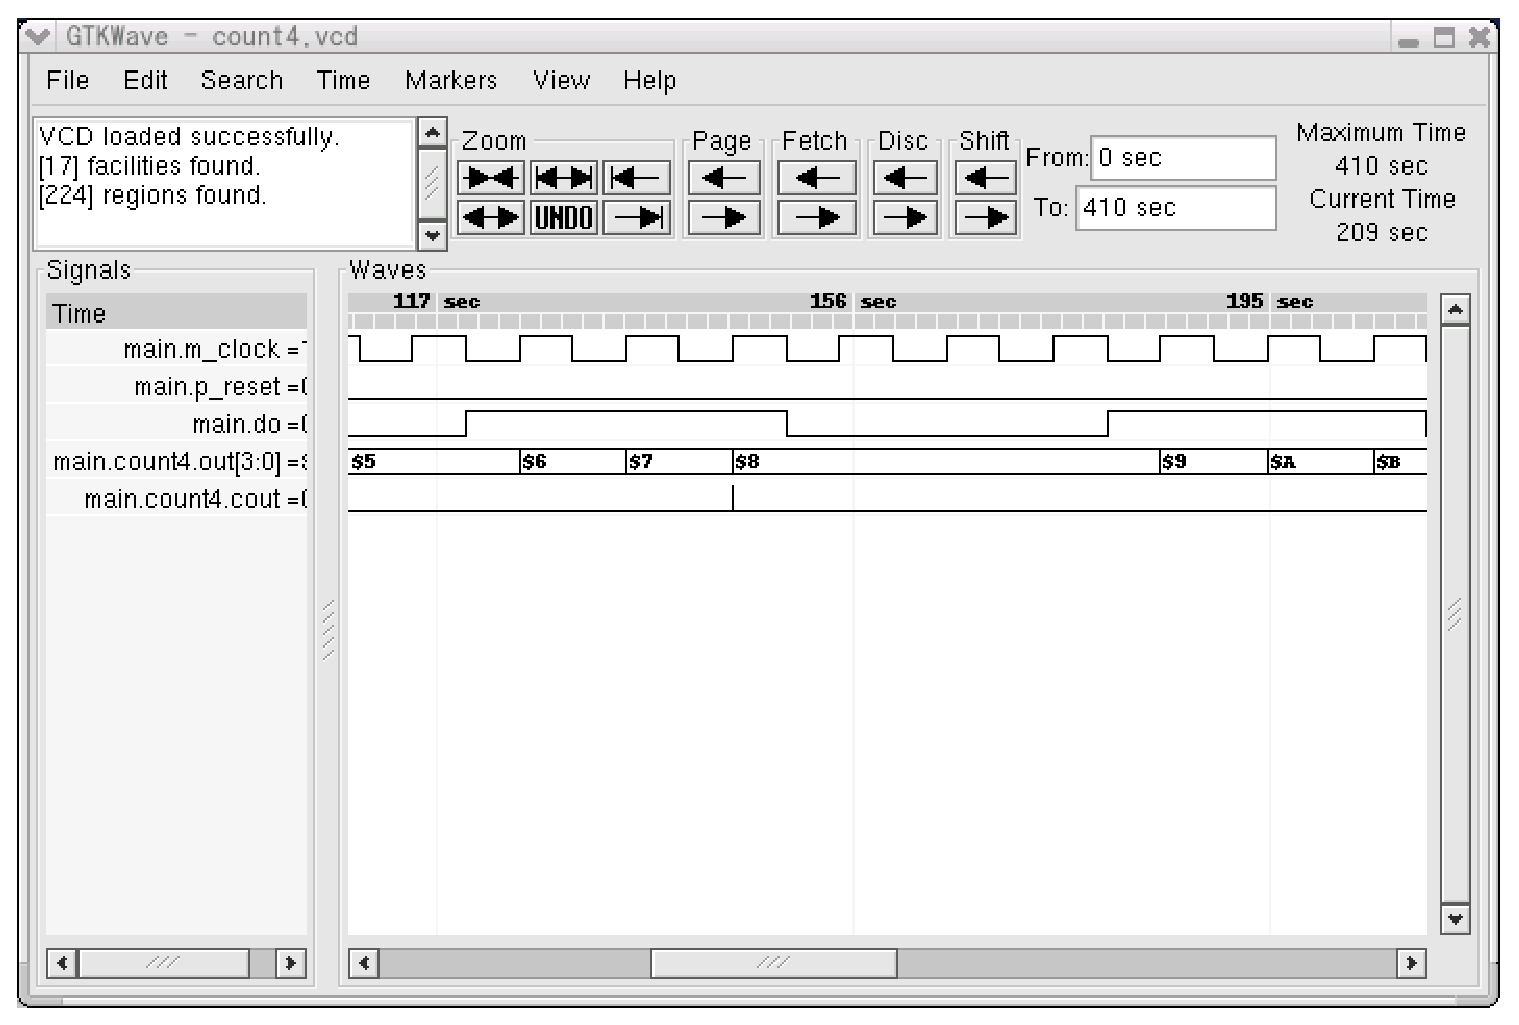
\includegraphics[scale=0.5]{count4_gtkwave.eps}
\caption{4ビットカウンタをシミュレーションした際の信号波形}
\label{fig:4ビットカウンタをシミュレーションした際の信号波形}
\end{center}
\end{figure}

\end{document}
